\chapter{Screenshot of Secure Data and Key Storage Scheme}
\label{app:screenshot}
Appendix body

% SRAM A
\begin{figure}[tph!]
    \centerline{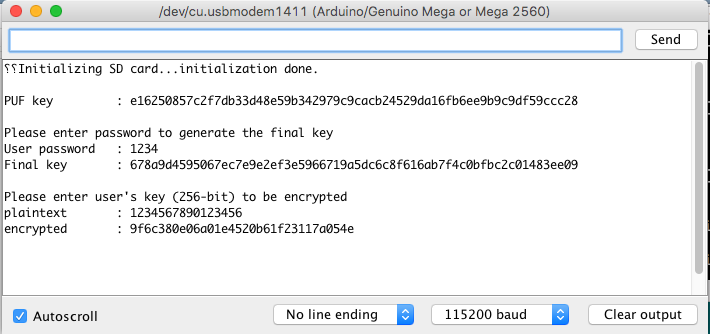
\includegraphics[width={\textwidth}]{images/A_encrypt}}
    \caption{Screenshot of the bitcoin key storing experiment during encryption stage using SRAM Cypress CY62256NLL 'A'.
    User's password is '1234' and the bitcoin key (user's key) is '1234567890123456'.}
    \label{fig:A_encrypt}
\end{figure}

\begin{figure}[tph!]
    \centerline{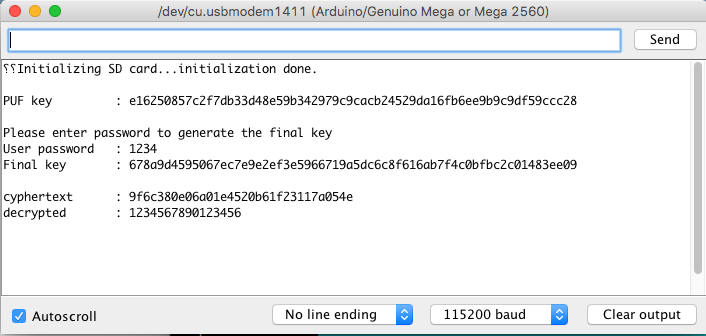
\includegraphics[width={\textwidth}]{images/A_decrypt_correct}}
    \caption{Screenshot of the bitcoin key storing experiment during decryption stage. The bitcoin key '1234567890123456' is previously secured by using SRAM Cypress CY62256NLL 'A' and user's password '1234'.
    The bitcoin key can be reconstructed because user's password is correct.}
    \label{fig:A_decrypt_correct}
\end{figure}

\begin{figure}[tph!]
    \centerline{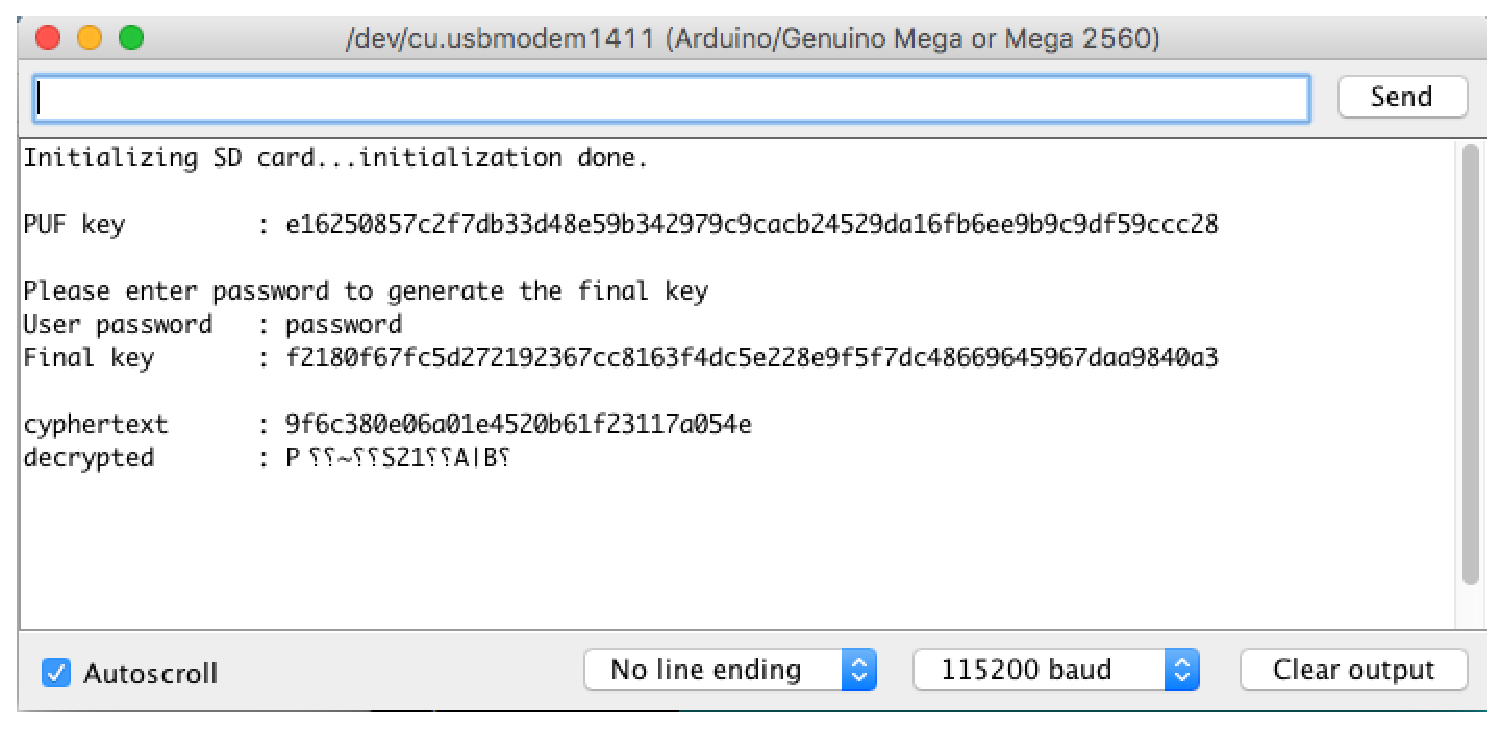
\includegraphics[width={\textwidth}]{images/A_decrypt_wrong_password}}
    \caption{Screenshot of the bitcoin key storing experiment during decryption stage. The bitcoin key '1234567890123456' is previously secured by using SRAM Cypress CY62256NLL 'A' and user's password '1234'.
    The bitcoin key cannot be reconstructed because user's password is wrong.}
    \label{fig:A_decrypt_wrong_password}
\end{figure}

\begin{figure}[tph!]
    \centerline{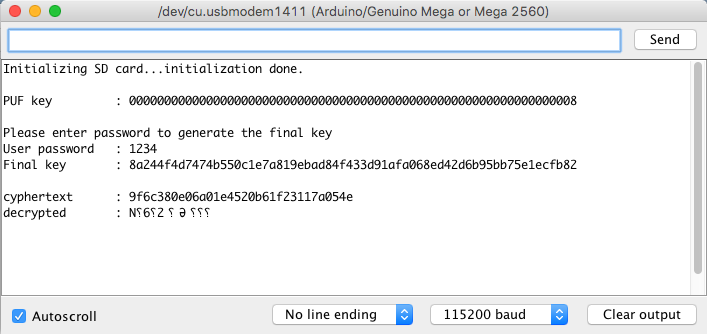
\includegraphics[width={\textwidth}]{images/A_decrypt_wrong_SRAM_D}}
    \caption{Screenshot of the bitcoin key storing experiment during decryption stage. The bitcoin key '1234567890123456' is previously secured by using SRAM Cypress CY62256NLL 'A' and user's password '1234'.
    The bitcoin key cannot be reconstructed because the SRAM utilized for the decryption is SRAM Cypress CY62256NLL 'D'.}
    \label{fig:A_decrypt_wrong_SRAM}
\end{figure}

% SRAM B
\begin{figure}[tph!]
    \centerline{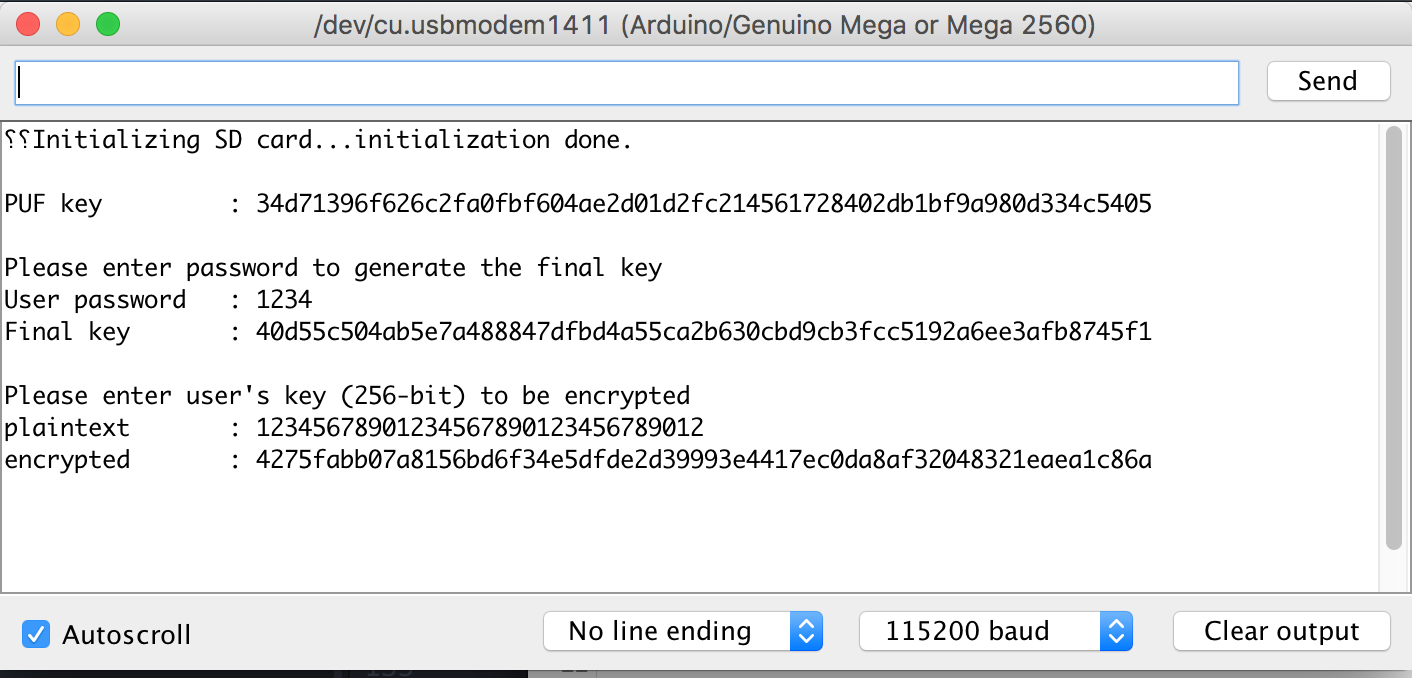
\includegraphics[width={\textwidth}]{images/B_encrypt}}
    \caption{Screenshot of the bitcoin key storing experiment during encryption stage using SRAM Cypress CY62256NLL 'B'.
    User's password is 'testpassword' and the bitcoin key (user's key) is 'testpasswordtest'.}
    \label{fig:B_encrypt}
\end{figure}

\begin{figure}[tph!]
    \centerline{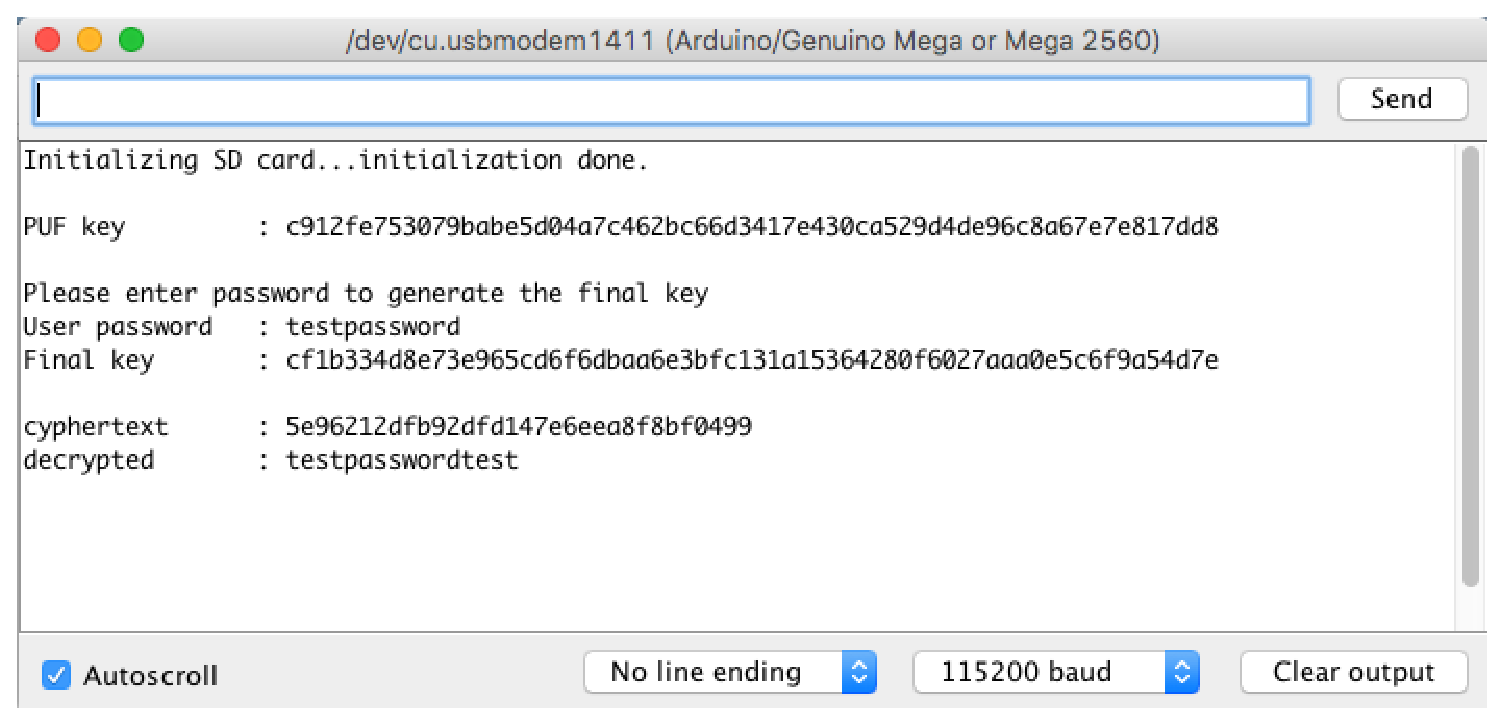
\includegraphics[width={\textwidth}]{images/B_decrypt_correct}}
    \caption{Screenshot of the bitcoin key storing experiment during decryption stage. The bitcoin key 'testpasswordtest' is previously secured by using SRAM Cypress CY62256NLL 'B' and user's password 'testpassword'.
    The bitcoin key can be reconstructed because user's password is correct.}
    \label{fig:B_decrypt_correct}
\end{figure}

\begin{figure}[tph!]
    \centerline{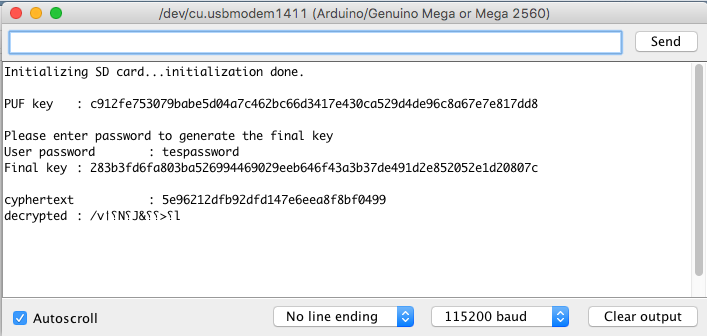
\includegraphics[width={\textwidth}]{images/B_decrypt_wrong_password}}
    \caption{Screenshot of the bitcoin key storing experiment during decryption stage. The bitcoin key 'testpasswordtest' is previously secured by using SRAM Cypress CY62256NLL 'B' and user's password 'testpassword'.
    The bitcoin key cannot be reconstructed because user's password is wrong.}
    \label{fig:B_decrypt_wrong_password}
\end{figure}

\begin{figure}[tph!]
    \centerline{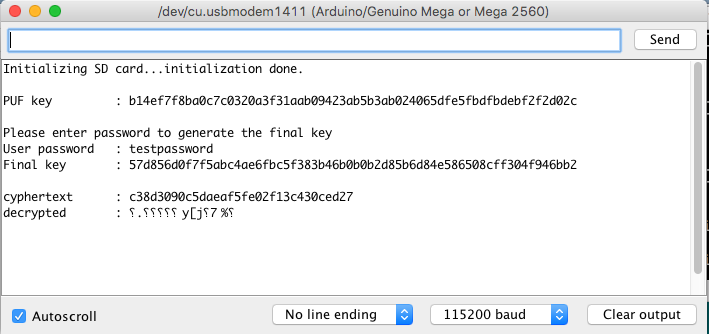
\includegraphics[width={\textwidth}]{images/B_decrypt_wrong_SRAM_A}}
    \caption{Screenshot of the bitcoin key storing experiment during decryption stage. The bitcoin key 'testpasswordtest' is previously secured by using SRAM Cypress CY62256NLL 'B' and user's password 'testpassword'.
    The bitcoin key cannot be reconstructed because the SRAM utilized for the decryption is SRAM Cypress CY62256NLL 'A'.}
    \label{fig:B_decrypt_wrong_SRAM}
\end{figure}

% SRAM C
\begin{figure}[tph!]
    \centerline{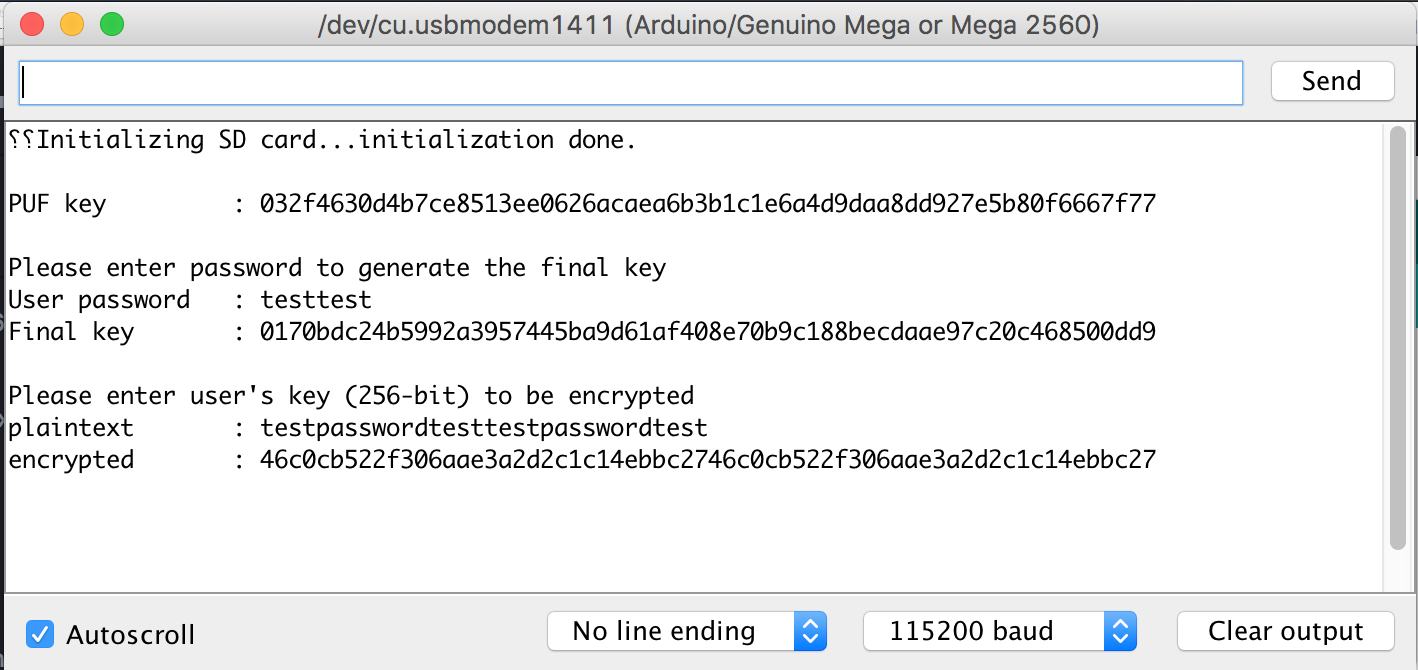
\includegraphics[width={\textwidth}]{images/C_encrypt}}
    \caption{Screenshot of the bitcoin key storing experiment during encryption stage using SRAM Cypress CY62256NLL 'C'.
    User's password is 'password' and the bitcoin key (user's key) is 'testpasswordtest'.}
    \label{fig:C_encrypt}
\end{figure}

\begin{figure}[tph!]
    \centerline{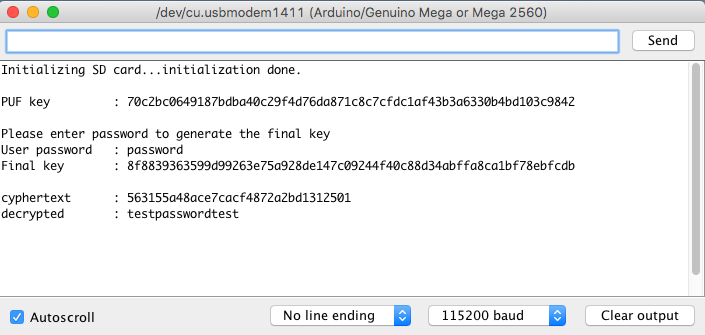
\includegraphics[width={\textwidth}]{images/C_decrypt_correct}}
    \caption{Screenshot of the bitcoin key storing experiment during decryption stage. The bitcoin key 'testpasswordtest' is previously secured by using SRAM Cypress CY62256NLL 'C' and user's password 'password'.
    The bitcoin key can be reconstructed because user's password is correct.}
    \label{fig:C_decrypt_correct}
\end{figure}

\begin{figure}[tph!]
    \centerline{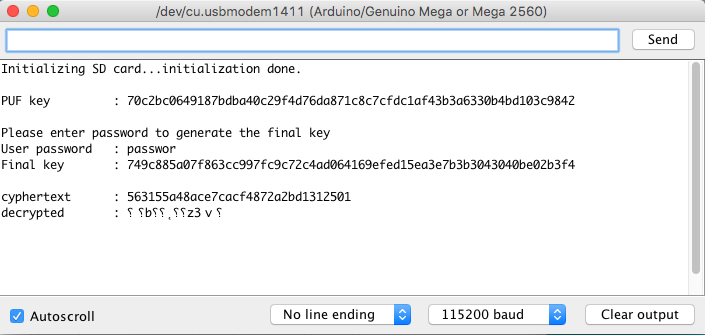
\includegraphics[width={\textwidth}]{images/C_decrypt_wrong_password}}
    \caption{Screenshot of the bitcoin key storing experiment during decryption stage. The bitcoin key 'testpasswordtest' is previously secured by using SRAM Cypress CY62256NLL 'C' and user's password 'password'.
    The bitcoin key cannot be reconstructed because user's password is wrong.}
    \label{fig:C_decrypt_wrong_password}
\end{figure}

\begin{figure}[tph!]
    \centerline{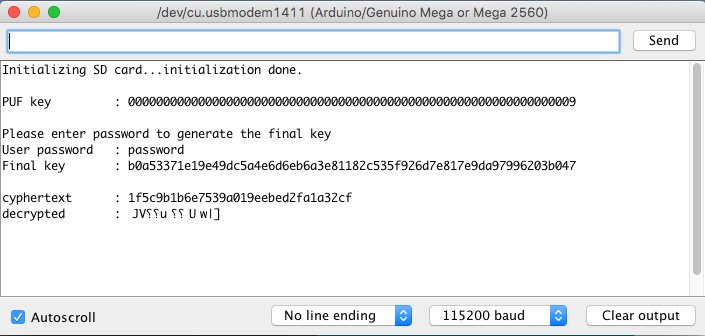
\includegraphics[width={\textwidth}]{images/C_decrypt_wrong_SRAM_D}}
    \caption{Screenshot of the bitcoin key storing experiment during decryption stage. The bitcoin key 'testpasswordtest' is previously secured by using SRAM Cypress CY62256NLL 'C' and user's password 'password'.
    The bitcoin key cannot be reconstructed because the SRAM utilized for the decryption is SRAM Cypress CY62256NLL 'D'.}
    \label{fig:C_decrypt_wrong_SRAM}
\end{figure}

% SRAM D
\begin{figure}[tph!]
    \centerline{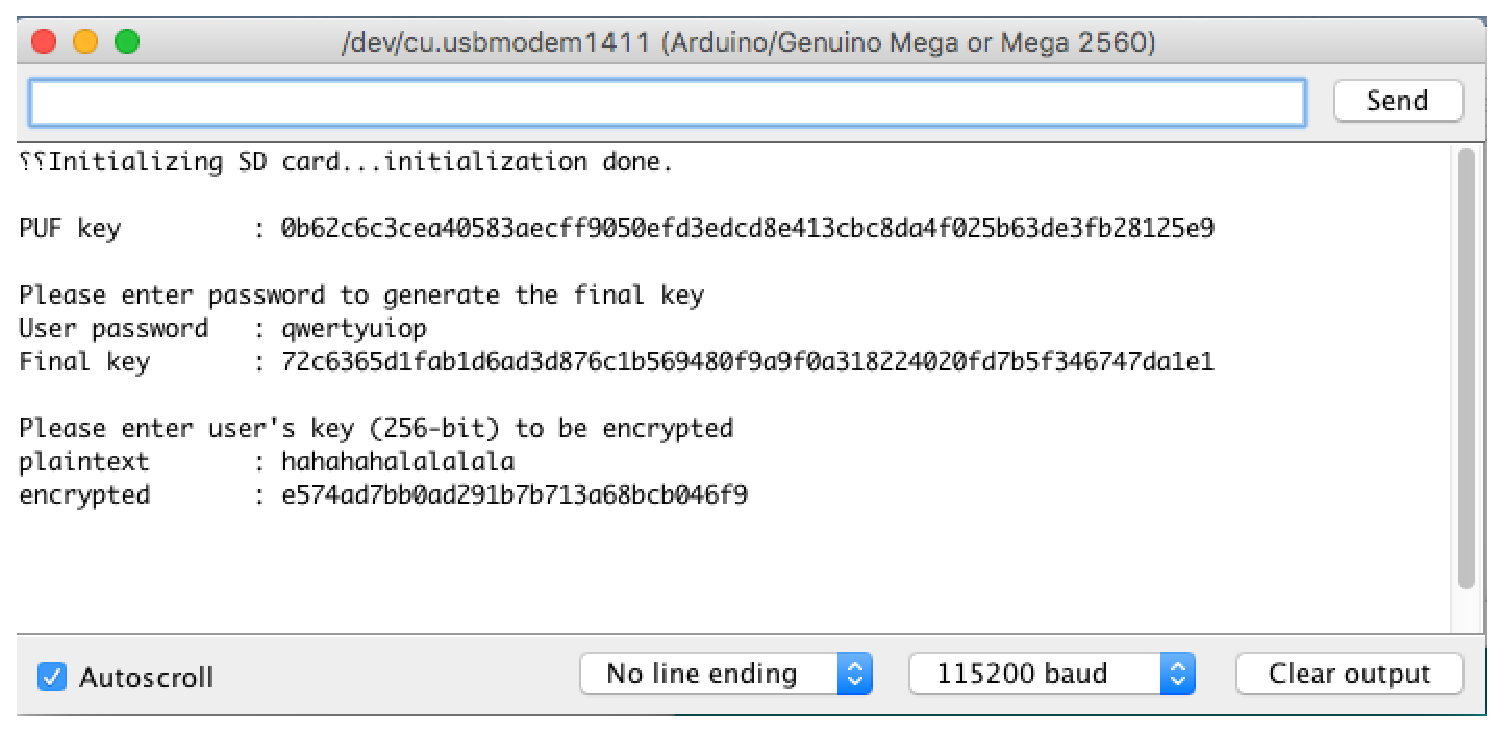
\includegraphics[width={\textwidth}]{images/D_encrypt}}
    \caption{Screenshot of the bitcoin key storing experiment during encryption stage using SRAM Cypress CY62256NLL 'D'.
    User's password is 'qwertyuiop' and the bitcoin key (user's key) is 'hahahahalalalala'.}
    \label{fig:D_encrypt}
\end{figure}

\begin{figure}[tph!]
    \centerline{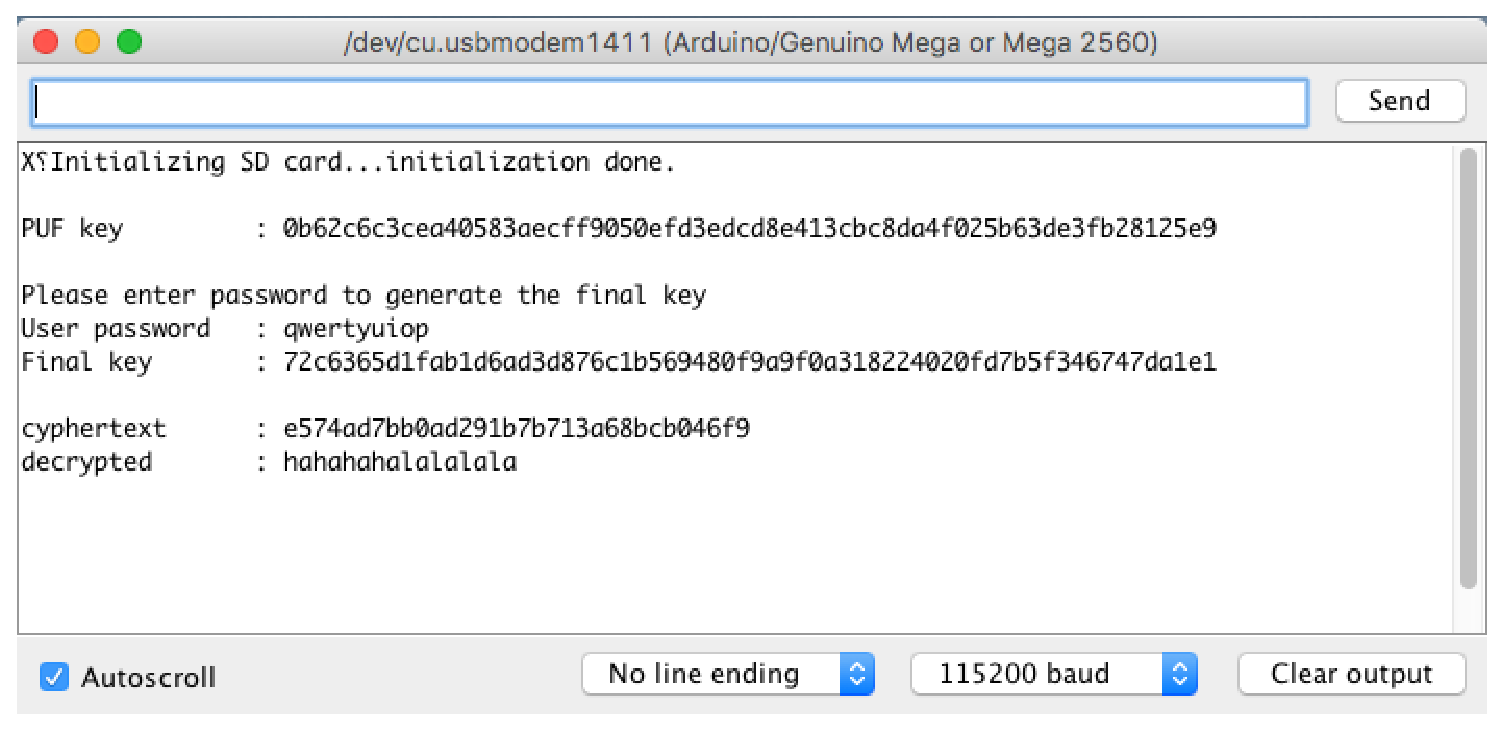
\includegraphics[width={\textwidth}]{images/D_decrypt_correct}}
    \caption{Screenshot of the bitcoin key storing experiment during decryption stage. The bitcoin key 'hahahahalalalala' is previously secured by using SRAM Cypress CY62256NLL 'D' and user's password 'qwertyuiop'.
    The bitcoin key can be reconstructed because user's password is correct.}
    \label{fig:D_decrypt_correct}
\end{figure}

\begin{figure}[tph!]
    \centerline{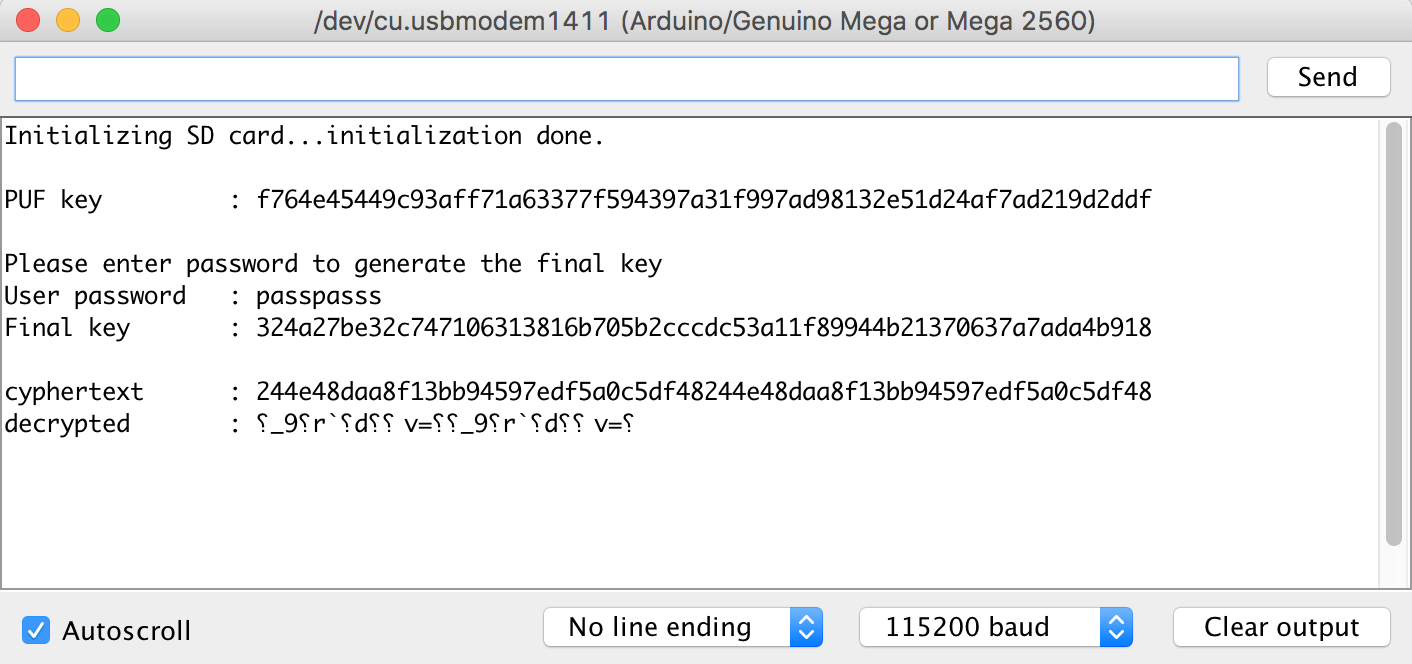
\includegraphics[width={\textwidth}]{images/D_decrypt_wrong_password}}
    \caption{Screenshot of the bitcoin key storing experiment during decryption stage. The bitcoin key 'hahahahalalalala' is previously secured by using SRAM Cypress CY62256NLL 'D' and user's password 'qwertyuiop'.
    The bitcoin key cannot be reconstructed because user's password is wrong.}
    \label{fig:D_decrypt_wrong_password}
\end{figure}

\begin{figure}[tph!]
    \centerline{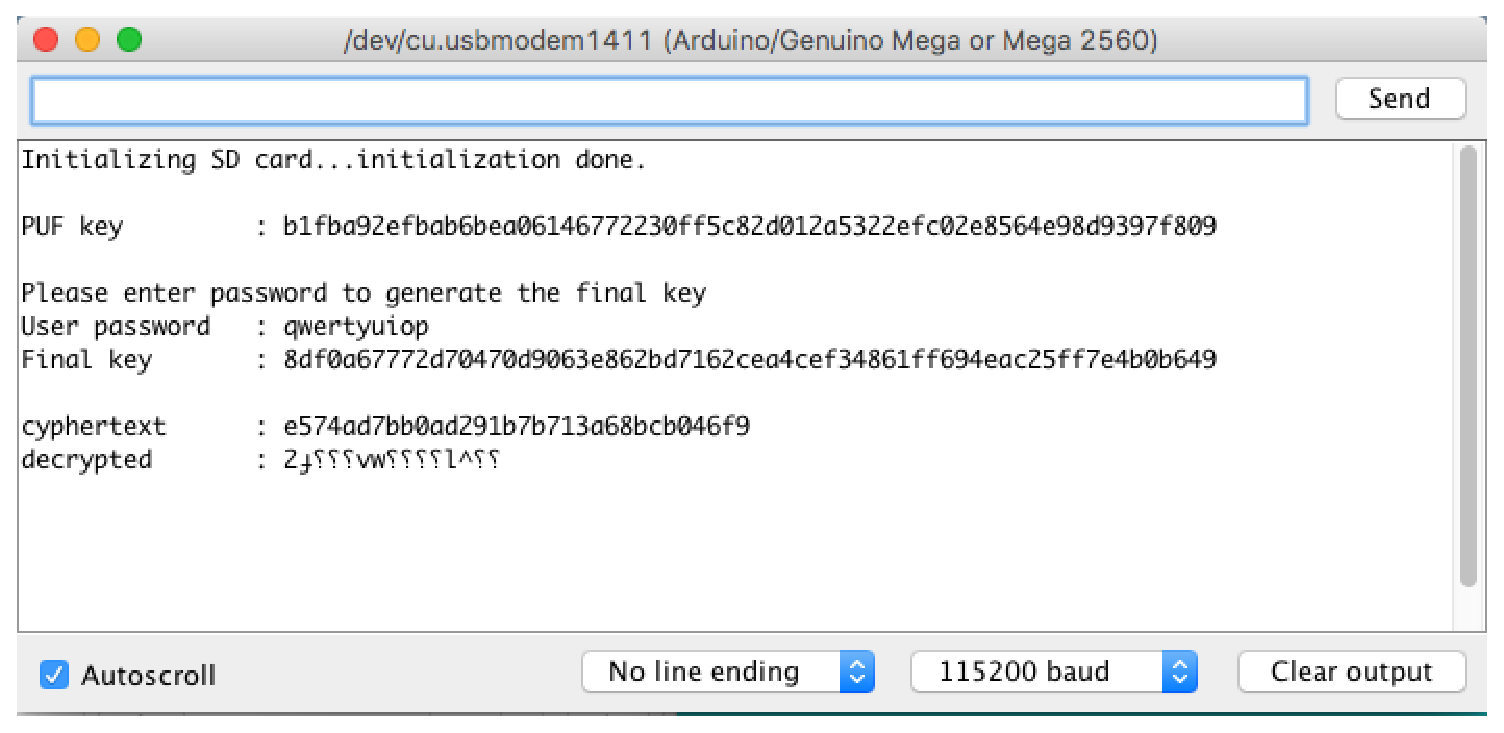
\includegraphics[width={\textwidth}]{images/D_decrypt_wrong_SRAM_B}}
    \caption{Screenshot of the bitcoin key storing experiment during decryption stage. The bitcoin key 'hahahahalalalala' is previously secured by using SRAM Cypress CY62256NLL 'D' and user's password 'qwertyuiop'.
    The bitcoin key cannot be reconstructed because the SRAM utilized for the decryption is SRAM Cypress CY62256NLL 'B'.}
    \label{fig:D_decrypt_wrong_SRAM}
\end{figure}

% SRAM E
\begin{figure}[tph!]
    \centerline{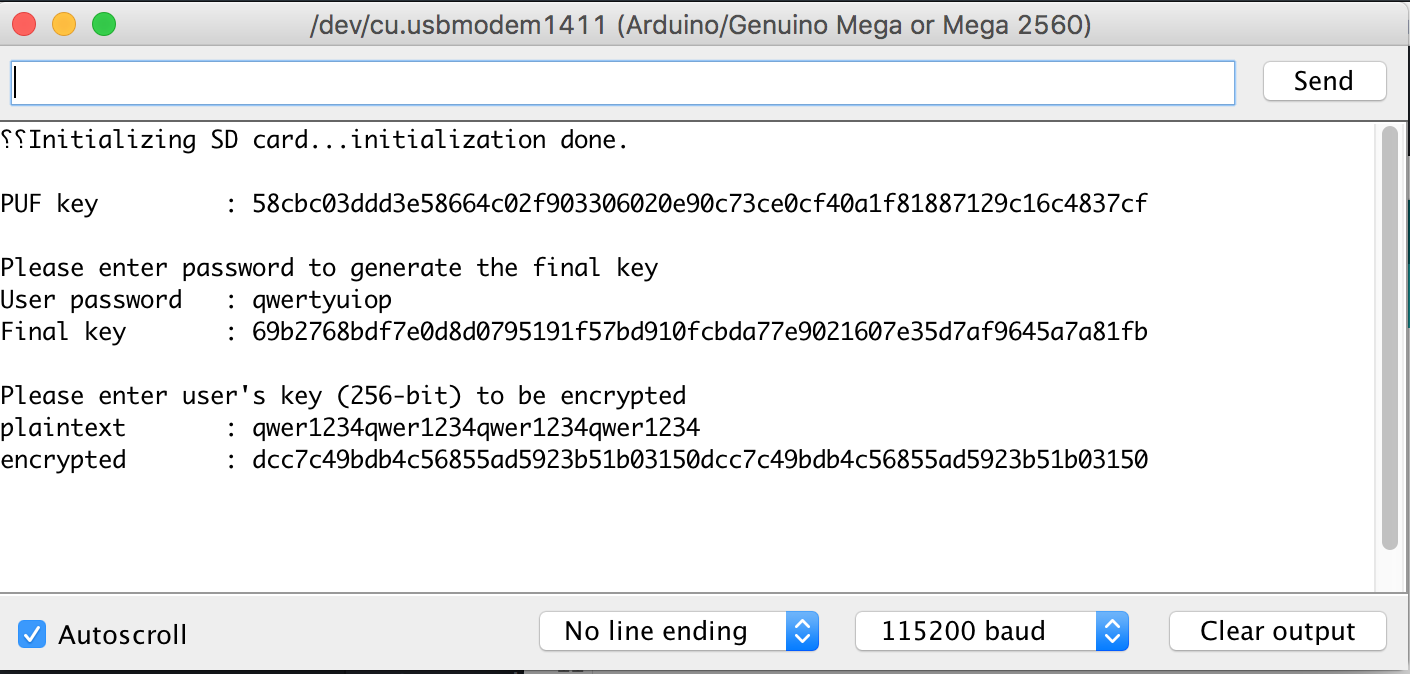
\includegraphics[width={\textwidth}]{images/E_encrypt}}
    \caption{Screenshot of the bitcoin key storing experiment during encryption stage using SRAM Cypress CY62256NLL 'E'.
    User's password is 'testtest' and the bitcoin key (user's key) is 'testpasswordtest'.}
    \label{fig:E_encrypt}
\end{figure}

\begin{figure}[tph!]
    \centerline{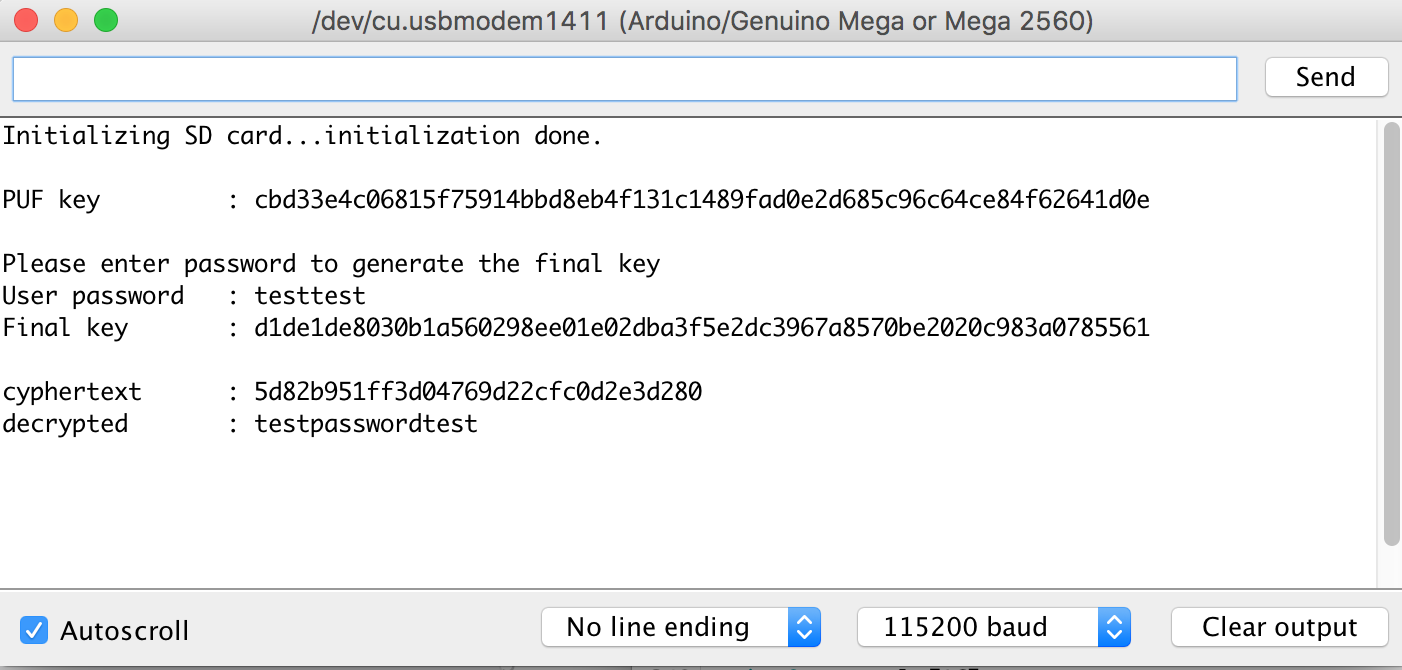
\includegraphics[width={\textwidth}]{images/E_decrypt_correct}}
    \caption{Screenshot of the bitcoin key storing experiment during decryption stage. The bitcoin key 'testpasswordtest' is previously secured by using SRAM Cypress CY62256NLL 'E' and user's password 'testtest'.
    The bitcoin key can be reconstructed because user's password is correct.}
    \label{fig:E_decrypt_correct}
\end{figure}

\begin{figure}[tph!]
    \centerline{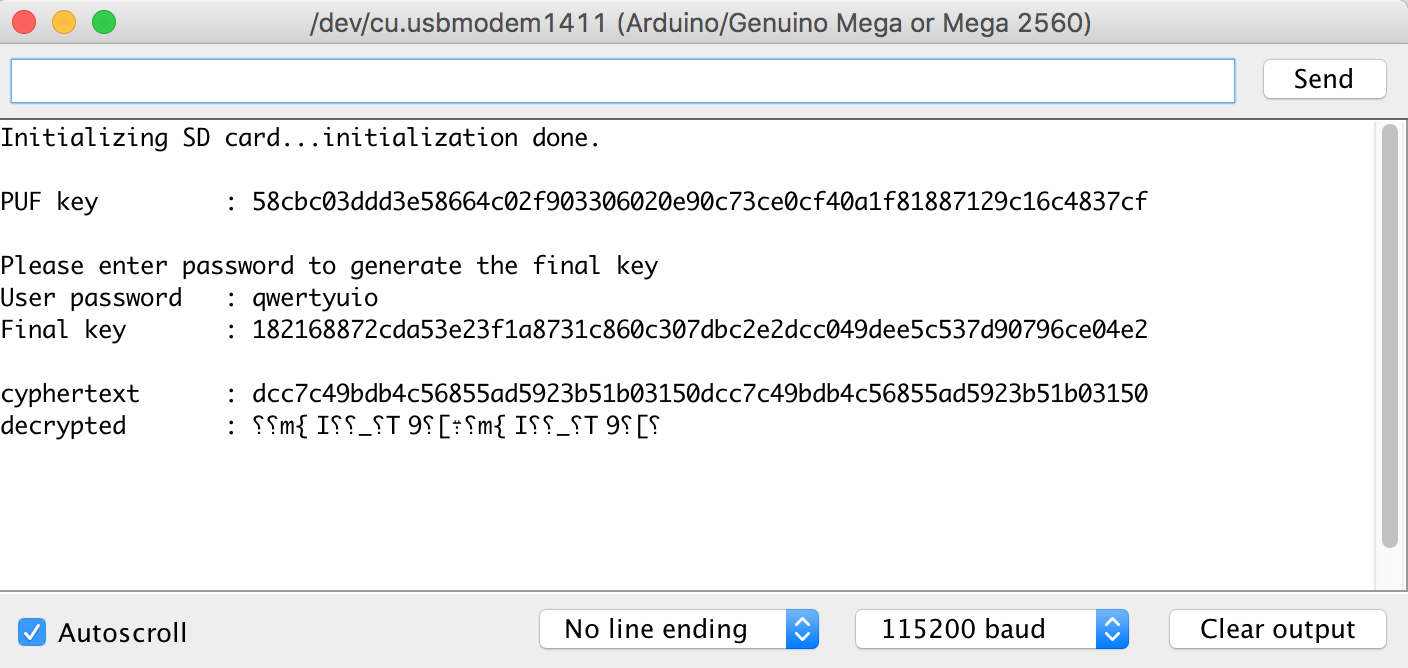
\includegraphics[width={\textwidth}]{images/E_decrypt_wrong_password}}
    \caption{Screenshot of the bitcoin key storing experiment during decryption stage. The bitcoin 'testpasswordtest' is previously secured by using SRAM Cypress CY62256NLL 'E' and user's password 'testtest'.
    The bitcoin key 'testpasswordtest' cannot be reconstructed because user's password is incorrect.}
    \label{fig:E_decrypt_wrong_password}
\end{figure}

\begin{figure}[tph!]
    \centerline{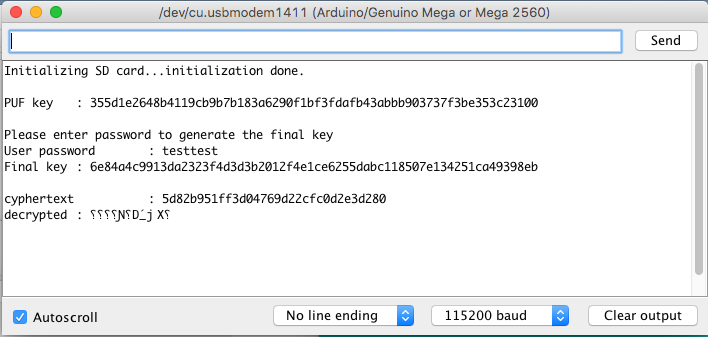
\includegraphics[width={\textwidth}]{images/E_decrypt_wrong_SRAM_C}}
    \caption{Screenshot of the bitcoin key storing experiment during decryption stage. The bitcoin key 'testpasswordtest' is previously secured by using SRAM Cypress CY62256NLL 'E' and user's password 'testtest'.
    The bitcoin key cannot be reconstructed because the SRAM utilized for the decryption is SRAM Cypress CY62256NLL 'C'.}
    \label{fig:E_decrypt_wrong_SRAM}
\end{figure}
